\documentclass[12pt,letterpaper]{article}
\usepackage{fullpage}
\usepackage[top=2cm, bottom=3.5cm, left=1.5cm, right=1.5cm]{geometry}
\usepackage{amsmath,amsthm,amsfonts,amssymb,amscd}
\usepackage{lastpage}
\usepackage{enumerate}
\usepackage{fancyhdr}
\usepackage{mathrsfs}
\usepackage{xcolor}
\usepackage{graphicx}
\usepackage{listings}
\usepackage{hyperref}
\usepackage{tikz}
\usepackage{enumitem}
\usepackage{circuitikz}
% packages for phasor
\usepackage{verbatim}
\usepackage{ifthen}
\usepackage{tikz}
\usepackage{pgf}
\usepackage{pgffor}
\usepgfmodule{shapes}
\usepgfmodule{plot}
\usetikzlibrary{decorations}
\usetikzlibrary{arrows}
\usetikzlibrary{snakes}
% setup for phasor
\usepackage{graphicx} % tablesgenerator.com
\usepackage{longtable}
% % % % % % % % % % % % % % % % % % % % % % % % % % % % % % % % % % % % % % % % 
\newcommand{\Gitter}[4]{
    \draw[very thin,color=gray] (#1,#3) grid (#2,#4);
}
\newcommand{\Koordinatenkreuz}[6]{
    \draw[->, >=latex, color=green!50!black] (#1,0) -- (#2,0) node[right] {#5};
    \draw[->, >=latex, color=green!50!black] (0,#3) -- (0,#4) node[left] {#6};
}
\newcommand{\KoordinatenkreuzOhneLabelsVerschobenKeinPfeil}[5]{
    \draw[-] (#1,0) -- (#2,0);
    \draw[-] (#5,#3) -- (#5,#4);
}
\newcommand{\ZeigerdiagrammText}[4]{
\begin{tikzpicture}[scale=.72, samples=100, >=latex]
    \def\Alpha{#1}
    \def\Phase{#2}
    \def\AmplitudeSpannung{#3}
    \def\AmplitudeStrom{#4}
    \def\SpannungsWert{{\AmplitudeSpannung*sin(\Alpha)}}
    \def\StromWert{{\AmplitudeStrom*sin(\Alpha+\Phase)}}
    \def\FarbeSpannung{blue!90!white}
    \def\FarbeStrom{red!90!white}
    \def\FarbeWinkelZeichnung{green}
    \def\Beta{\Alpha+\Phase}
    \def\AlphaRad{\Alpha*3.141592654/180}
    \def\PhaseRad{\Phase*3.141592654/180}
    \Gitter{-.1}{7.1}{-3.1}{3.1}
    \Koordinatenkreuz{-.2}{7.3}{-3.2}{3.3}{$\omega t$}{}
    \draw (1.570795,0) node[below]{$\frac{\pi}{2}$};
    \draw (3.14159,0) node[below]{${\pi}$};
    \draw (4.71238898,0) node[below]{$\frac{3\pi}{2}$};
    \draw (6.283185307,0) node[below]{${2\pi}$};
    \draw (-4,0) circle (3cm);
    \KoordinatenkreuzOhneLabelsVerschobenKeinPfeil{-7.2}{-.8}{-3.6}{3.6}{-4}
    % voltage
    \draw[color=\FarbeSpannung, very thick] plot[id=voltage, domain=0:7] function{\AmplitudeSpannung*sin(x)} node[right] {$V(t)$};
    % voltage circle
    \draw[color=\FarbeSpannung, loosely dashed] (-4,0) circle (\AmplitudeSpannung cm);
    % angle
    \draw[color=\FarbeWinkelZeichnung!50!black, thick] (\AlphaRad, \SpannungsWert)--(\AlphaRad,\StromWert) node[below=18pt] {$\alpha$};
    % angle in the circle
    \filldraw[fill=\FarbeWinkelZeichnung!20,draw=\FarbeWinkelZeichnung!50!black] (-4,0) -- (-3,0) arc (0:\Alpha:1) -- cycle node[right] {$\alpha$};
    % voltage pointer
    \draw[<-,color=\FarbeSpannung, very thick] (\Alpha:\AmplitudeSpannung)++(-4,0) --(-4,0)9
    \draw[color=\FarbeSpannung,  dashed] (\Alpha:\AmplitudeSpannung)++(-4,0) -- (\AlphaRad,\SpannungsWert);
    % current
    \draw[color=\FarbeStrom, very thick] plot[id=current, domain=0:7] function{\AmplitudeStrom*sin(x+\PhaseRad)} node[right] {$I(t)$};		
    % current circle
    \draw[color=\FarbeStrom, loosely dashed]    (-4,0) circle (\AmplitudeStrom cm);
    % current pointer
    \draw[<-,color=\FarbeStrom, very thick] (\Beta:\AmplitudeStrom)++(-4,0) --(-4,0);
    \draw[color=\FarbeStrom, dashed](\Beta:\AmplitudeStrom)++(-4,0) -- (\AlphaRad,\StromWert);
    % phase difference
    \ifthenelse{\Phase<0}{
        \draw[snake=brace] (pi/2 ,3.3)--(pi/2-\PhaseRad ,3.3) node[above=7pt, left=10pt] {$\phi$};
    }
    {
        \draw[snake=brace] (pi/2-\PhaseRad ,3.3)--(pi/2 ,3.3) node[above=7pt, left=10pt] {$\phi$};
    }
    % angular velocity \omega
    \draw[->, xshift=-4cm]  (120:2.4cm) arc (120:170:2) node[below] {$\omega$};
\end{tikzpicture}
}
%end of phasor

\hypersetup{
  colorlinks=true,
  linkcolor=blue,
  linkbordercolor={0 0 1}
}
 
\renewcommand\lstlistingname{Code}
\renewcommand\lstlistlistingname{Code}
\def\lstlistingautorefname{Code}

\lstdefinestyle{Bash}{
    language        = Bash,
    frame           = lines, 
    basicstyle      = \footnotesize,
    keywordstyle    = \color{blue},
    stringstyle     = \color{brown},
    commentstyle    = \color{red}\ttfamily
}
\setlength{\parindent}{0.0in}
\setlength{\parskip}{0.05in}

\newcommand\course{POWER SYSTEMS CONTROL OPERATOR I/II}

\pagestyle{fancyplain}
\headheight 35pt
\lhead{\NetIDa}
\chead{\textbf{\Large Candidate Assessment}}
\rhead{\course \\ \today}
\lfoot{}
\cfoot{}
\rfoot{\small\thepage}
\headsep  0.5em

\begin{document}

CANDIDATE NAME:\\
START TIME:\\
END TIME:\\
\section*{Technical Knowledge}
This section is designed to assess your technical abilities. Please answer all questions as best as you can. DO NOT BE DISCOURAGED IF YOU ARE UNABLE TO ANSWER A QUESTION OR IF YOU RUN OUT OF TIME. This portion of the assessment is closed to any outside resources and the time limit is 20 minutes. Please return this assessment to your proctor when finished.  
\begin{enumerate}[itemsep=50pt,parsep=2pt]
\item
Describe power factor, how it is calculated, as well as its significance in AC circuits.
\item Assuming a three-phase AC circuit, label each plot as being either an INDUCTIVE LOAD, a CAPACITIVE LOAD, or a RESISTIVE LOAD. Hint: ELI the ICE Man
    \begin{enumerate}
      \item
            \ZeigerdiagrammText{60}{0}{2.7}{1.8}\\
            INDUCTIVE, CAPACITIVE, or RESISTIVE load (circle one)
      \item
          \ZeigerdiagrammText{60}{-90}{2.7}{1.8}\\
            INDUCTIVE, CAPACITIVE, or RESISTIVE load (circle one)
       \item
          \ZeigerdiagrammText{60}{90}{2.7}{1.8}\\
            INDUCTIVE, CAPACITIVE, or RESISTIVE load (circle one)
    \end{enumerate}
\item Given the following simplified AC circuit:
    \begin{equation}
\begin{circuitikz}[xscale = 1]
\draw
(2,0) to[sinusoidal voltage source, label=$60Hz$] (4,0)
(4,0) to[L] (8,0)
(4,0) to[short] (8,0)
(5.55,0) to[short] (5.55,-1.5)
(6.5,0) to[short] (6.5,-1.5)
(5.55,-1.5) to[ammeter,label=$A_1$] (6.5,-1.5)
(9,0) node[transformer] (T) {}
(T.A1) node[anchor=east] {}
(T.A2) node[anchor=east] {}
(T.B1) node[anchor=west] {}
(T.B2) node[anchor=west] {}
(T.A2) to[short] (2,-2.1)
(T.base) node{$T_1$}
(2,-2.1) to[short] (2,0)
(T.B1) to[voltmeter,label=$V_1$] (12,0)
(12,0) to[short] (12,-2.1)
(12,-2.1) to[short] (T.B2)
;
\end{circuitikz}
    \end{equation}
\begin{enumerate}[itemsep=50pt,parsep=2pt]
    \item Identify the potential transformer (PT). What does a PT measure?
    \item Identify the current transformer (CT). What does a CT measure?
\end{enumerate}
\item
What is the functional difference between TELEMETRY/ANALOG data and STATUS/BINARY/DIGITAL data? Please give an example for each type of data.
\pagebreak
\item Describe what the following code is does as well expected output.
\begin{lstlisting}[style = Bash]
#!/bin/bash
for i in Alfonso Tad Michal Travis Slim-Shady
do
   echo "My name is $i"
done
    \end{lstlisting}
    \begin{enumerate} [itemsep=50pt,parsep=2pt]
        \item What does this script do?
        \item What is the expected output?
    \end{enumerate}
     
  \item Given the following power triangle where A is a right angle,
\begin{center}
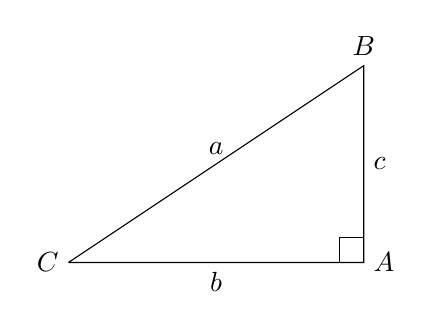
\begin{tikzpicture}[centered, scale=1.25]%,cap=round,>=latex]
\coordinate [label=left:$C$] (A) at (-1.5cm,-1.cm);
\coordinate [label=right:$A$] (C) at (1.5cm,-1.0cm);
\coordinate [label=above:$B$] (B) at (1.5cm,1.0cm);
\draw (A) -- node[above] {$a$} (B) -- node[right] {$c$} (C) -- node[below] {$b$} (A);
\draw (1.25cm,-1.0cm) rectangle (1.5cm,-0.75cm);
\end{tikzpicture}
\end{center}\\
Side a is the \underline{\hspace{3cm}}, measured in (units)\underline{\hspace{3cm}};\\
Side b is the \underline{\hspace{3cm}}, measured in (units)\underline{\hspace{3cm}};\\
Side c is the \underline{\hspace{3cm}}, measured in (units)\underline{\hspace{3cm}};\\
Cosine of angle C is the \underline{\hspace{3cm}}.\\
Available choices include: True Power, Reactive Power, Apparent Power, Watts (W), Volt-Amps (VA), Volt-Amps Reactive (VAR), Power Factor (PF)
\item In power systems calculations, if P=I*E then:\\
P is the \underline{\hspace{3cm}}, measured in (units)\underline{\hspace{3cm}};\\
I is the \underline{\hspace{3cm}}, measured in (units)\underline{\hspace{3cm}};\\
E is the \underline{\hspace{3cm}}, measured in (units)\underline{\hspace{3cm}};\\
Available choices include: Current, Voltage, Impedance, Energy, Power, Potential, Volts, Vars, KVar, Amps, Watts
\end{enumerate}
\begin{center}
    \textbf{*** PLEASE RETURN THIS PORTION OF THE ASSESSMENT TO THE PROCTOR BEFORE PROCEEDING TO THE NEXT SECTION. ***}
\end{center}
\pagebreak
\section*{Spreadsheets}
This section will assess your ability to manipulate data. Provo Power Dispatchers are tasked with creating reports and interpreting data from multiple various sources. One of the most efficient, clean, and effective ways to move data between systems is by a Comma Separated Value (CSV) file.\\
On the thumb drive that you were given you will find a file named 'DataSet.csv'. This data set is real data that was stored by our SCADA system and comprises the Provo Power 15 minute peak system demand for 6/21/2019. With this data, please complete the following tasks:
\begin{enumerate}
    \item Import the data into Excel or LibreCalc.
    \item Organize the data in any way that helps the data 'tell a story'. Some of the functions that you might want to use are: Sort, Average, Sum, Minimum, Maximum, etc. Be creative and find interesting ways to present this data.
    \item Style your data as you see fit.
    \item Save the output of your work on the same thumb drive and name it DataSet[YOURNAME].xlsx
    \item When finished, return the thumb drive to the proctor. 
\end{enumerate}
This section is designed to not only test your current knowledge and skills, but to also to test your ability to figure something out. You are allowed to use any resources available to you with the exception of having someone do this work for you. The maximum time allowed to complete and submit this assignment is 20 minutes.
\begin{table}[]
\resizebox{\textwidth}{!}{%
\begin{tabular}{llllll}
\hline
\textbf{Time} & \textbf{System Demand} & \textbf{RMP Interconnect Demand} & \textbf{Generation Into System} & \textbf{Olmsted Generation} & \textbf{UMPA Generation} \\ \hline
12:15 AM      & 60.7793730692269       & 51.0293733962808                 & -9.74999967294608               & -9.74999967294608           & 0                        \\
12:30 AM      & 59.4632793277307       & 49.7132796547847                 & -9.74999967294608               & -9.74999967294608           & 0                        \\
12:45 AM      & 57.7974199929489       & 48.0474203200028                 & -9.74999967294608               & -9.74999967294608           & 0                        \\
01:00 AM      & 56.0364825412168       & 46.2964828679353                 & -9.73999967328152               & -9.73999967328152           & 0                        \\
01:15 AM      & 55.0482794412643       & 45.3082797679828                 & -9.73999967328152               & -9.73999967328152           & 0                        \\
01:30 AM      & 54.0902325805794       & 44.3402329076334                 & -9.74999967294608               & -9.74999967294608           & 0                        \\
01:45 AM      & 53.3782013425827       & 43.6082016703075                 & -9.7699996722752                & -9.7699996722752            & 0                        \\
02:00 AM      & 52.4360138720273       & 42.6860141990812                 & -9.74999967294608               & -9.74999967294608           & 0                        \\
02:15 AM      & 52.1923419916998       & 42.4323423190891                 & -9.75999967261064               & -9.75999967261064           & 0                        \\
02:30 AM      & 51.2579670187221       & 41.5179673454405                 & -9.73999967328152               & -9.73999967328152           & 0                        \\
02:45 AM      & 50.6581232791223       & 40.9181236058408                 & -9.73999967328152               & -9.73999967328152           & 0                        \\
03:00 AM      & 50.445388908558        & 40.7053892352765                 & -9.73999967328152               & -9.73999967328152           & 0                        \\
03:15 AM      & 50.410467029869        & 40.6704673565875                 & -9.73999967328152               & -9.73999967328152           & 0                        \\
03:30 AM      & 50.4732014054649       & 40.7132017328543                 & -9.75999967261064               & -9.75999967261064           & 0                        \\
03:45 AM      & 50.6848420249858       & 40.9248423523751                 & -9.75999967261064               & -9.75999967261064           & 0                        \\
04:00 AM      & 49.8641389366963       & 40.1141392637502                 & -9.74999967294608               & -9.74999967294608           & 0                        \\
04:15 AM      & 50.331638938296        & 40.5816392653499                 & -9.74999967294608               & -9.74999967294608           & 0                        \\
04:30 AM      & 50.4843733108729       & 40.7443736375914                 & -9.73999967328152               & -9.73999967328152           & 0                        \\
04:45 AM      & 50.9220295537529       & 41.1720298808068                 & -9.74999967294608               & -9.74999967294608           & 0                        \\
05:00 AM      & 51.5184357999485       & 41.7684361270024                 & -9.74999967294608               & -9.74999967294608           & 0                        \\
05:15 AM      & 52.6803107825765       & 42.9303111096304                 & -9.74999967294608               & -9.74999967294608           & 0                        \\
05:30 AM      & 53.416717024076        & 43.6767173507945                 & -9.73999967328152               & -9.73999967328152           & 0                        \\
05:45 AM      & 54.3582013788359       & 44.6182017055544                 & -9.73999967328152               & -9.73999967328152           & 0                        \\
06:00 AM      & 54.2136701390845       & 44.473670465803                  & -9.73999967328152               & -9.73999967328152           & 0                        \\
06:15 AM      & 55.473904491793        & 45.7339048185115                 & -9.73999967328152               & -9.73999967328152           & 0                        \\
06:30 AM      & 55.6160919891837       & 45.8660923162376                 & -9.74999967294608               & -9.74999967294608           & 0                        \\
06:45 AM      & 56.6901544769175       & 46.9401548039714                 & -9.74999967294608               & -9.74999967294608           & 0                        \\
07:00 AM      & 58.2731231965005       & 48.5231235235544                 & -9.74999967294608               & -9.74999967294608           & 0                        \\
07:15 AM      & 59.864060653935        & 50.1440609799826                 & -9.7199996739524                & -9.7199996739524            & 0                        \\
07:30 AM      & 60.7621075166326       & 51.0221078433511                 & -9.73999967328152               & -9.73999967328152           & 0                        \\
07:45 AM      & 63.1681230668657       & 53.4181233939197                 & -9.74999967294608               & -9.74999967294608           & 0                        \\
08:00 AM      & 65.4591386555196       & 55.7191389822381                 & -9.73999967328152               & -9.73999967328152           & 0                        \\
08:15 AM      & 66.4430449059985       & 56.7130452323815                 & -9.72999967361696               & -9.72999967361696           & 0                        \\
08:30 AM      & 68.8649198463611       & 59.1249201730795                 & -9.73999967328152               & -9.73999967328152           & 0                        \\
08:45 AM      & 69.7349979718779       & 60.0049982982609                 & -9.72999967361696               & -9.72999967361696           & 0                        \\
09:00 AM      & 70.8128885882636       & 61.0928889143112                 & -9.7199996739524                & -9.7199996739524            & 0                        \\
09:15 AM      & 72.0496854482389       & 62.3296857742865                 & -9.7199996739524                & -9.7199996739524            & 0                        \\
09:30 AM      & 71.9993729693683       & 62.4293732903843                 & -9.569999678984                 & -9.569999678984             & 0                        \\
09:45 AM      & 73.134294811159        & 63.5342951331813                 & -9.59999967797768               & -9.59999967797768           & 0                        \\
10:00 AM      & 74.1752322870427       & 64.5652326094005                 & -9.60999967764224               & -9.60999967764224           & 0                        \\
10:15 AM      & 75.4698416429186       & 65.8698419649409                 & -9.59999967797768               & -9.59999967797768           & 0                        \\
10:30 AM      & 75.902966641351        & 66.2929669637088                 & -9.60999967764224               & -9.60999967764224           & 0                        \\
10:45 AM      & 77.1518728483776       & 67.5018731720771                 & -9.64999967630048               & -9.64999967630048           & 0                        \\
11:00 AM      & 77.641872831941        & 68.0118731549697                 & -9.62999967697136               & -9.62999967697136           & 0                        \\
11:15 AM      & 77.8464822243798       & 68.2064825477439                 & -9.63999967663592               & -9.63999967663592           & 0                        \\
11:30 AM      & 78.0541384749749       & 68.4041387986744                 & -9.64999967630048               & -9.64999967630048           & 0                        \\
11:45 AM      & 78.235935335776        & 68.6059356588046                 & -9.62999967697136               & -9.62999967697136           & 0                        \\
12:00 PM      & 77.796482226057        & 68.1664825490857                 & -9.62999967697136               & -9.62999967697136           & 0                        \\
 \hline
\end{tabular}%
}
\caption{DataSet.csv (partial)}
\label{tab:my-table}
\end{table}
\end{document}
